\documentclass{standalone}
\usepackage{tikz}
\begin{document}

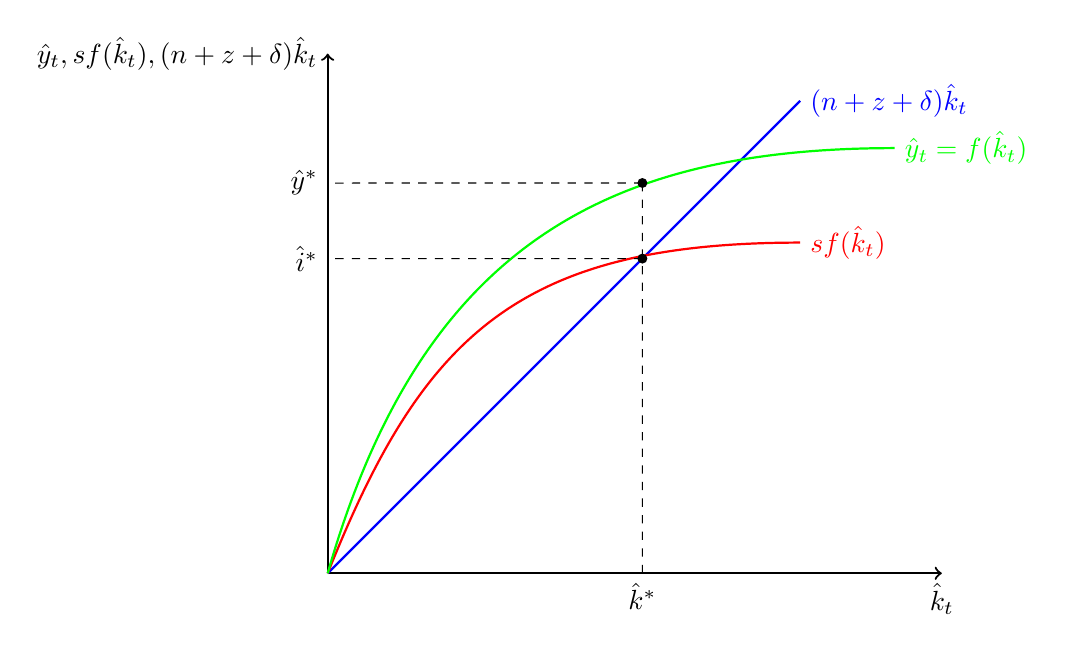
\begin{tikzpicture}[scale=1.2, domain=0:6]
  % Axes
  \draw[thick, ->] (0,0) node[below left] {} -- (6.5,0) node[below] {$\hat{k}_{t}$};
  \draw[thick, ->] (0,0) -- (0,5.5) node[left] {$\hat{y}_{t}, sf(\hat{k}_t), (n+z+\delta)\hat{k}_{t}$};

  % Depreciation line ( \delta k )
  \draw[thick, blue] (0,0) -- (5,5) node[right] {$(n+z+\delta)\hat{k}_{t}$};

  % Saving curve ( sf(k) )
  \draw[thick, red] (0,0) .. controls (1,2.5) and (2,3.5) .. (5,3.5) node[right] {$sf(\hat{k}_{t})$};

  % Saving curve ( sf(k) )
  \draw[thick, green] (0,0) .. controls (1,3.5) and (3,4.5) .. (6,4.5) node[right] {$\hat{y}_{t} = f(\hat{k}_{t})$};

  % Steady state markers
  \coordinate (SS1) at (3.33, 3.33);
  \coordinate (SS2) at (3.33, 4.13);
  \fill[black] (SS1) circle (1.5pt);
  \fill[black] (SS2) circle (1.5pt);
  \draw[dashed] (SS2) -- (3.33,0) node[below] {$\hat{k}^*$};
  \draw[dashed] (SS1) -- (0,3.33) node[left] {$\hat{i}^*$};
  \draw[dashed] (SS2) -- (0,4.13) node[left] {$\hat{y}^*$};
\end{tikzpicture}

\end{document}